\begin{figure}[htpb]
  \centering
  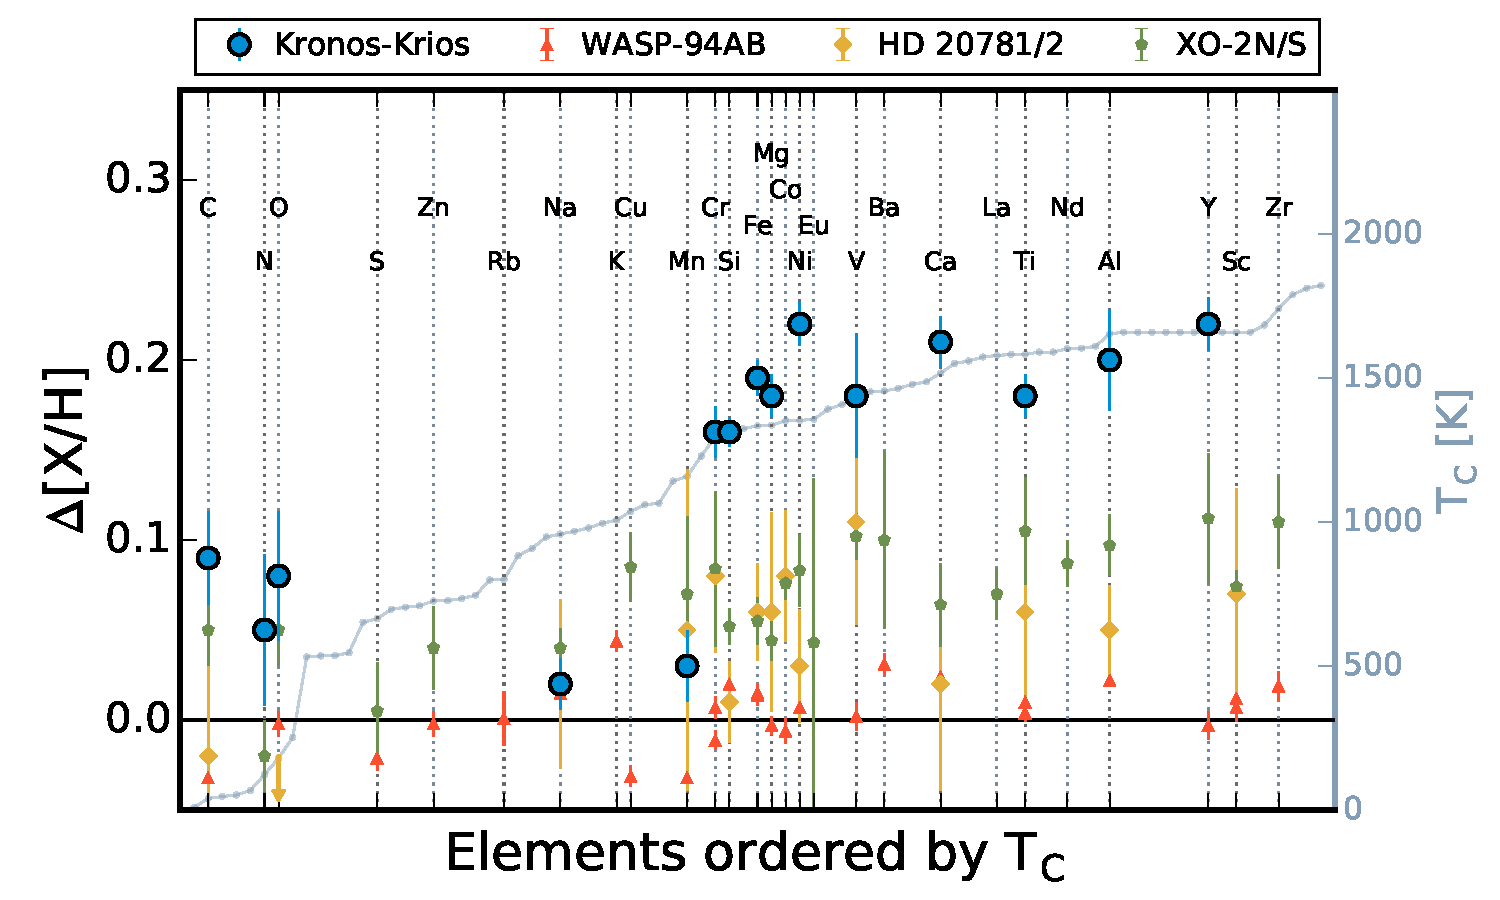
\includegraphics[width=0.95\linewidth]{TcRank_deltaXH_concise.pdf}
  \caption{Abundance differences of the \bizarreone-\sunanalog\ pair
    ranked by the condensation temperature of elements for solar composition gas
    from \citealt{2003ApJ...591.1220L}.
    The condensation temperature may be read from the gray line and right y-axis.
    We show three wide binary systems selected from the literature:
    HD~20782/1 (\citealt{Mack:2014aa}, $\feh\approx0$),
    XO-2N/S (\citealt{Biazzo:2015aa}, $\feh\approx0.35$),
    and WASP-94AB (\citealt{Teske:2016aa}, $\feh\approx0.3$).
    Locations of elements with at least one measurement from any study
    are indicated by a vertical line and its symbol.
    Note that often multiple values are reported for one element corresponding
    to different ionization states in equivalent width analyses.
    No other pair studied so far were shown to have such large difference
    in metallicity or sharp contrast between (moderately) volatile and
    refractory elements as \bizarreone-\sunanalog.
  }
  \label{fig:relabun_tcrank}
\end{figure}


\begin{figure}[htbp]
  \begin{center}
    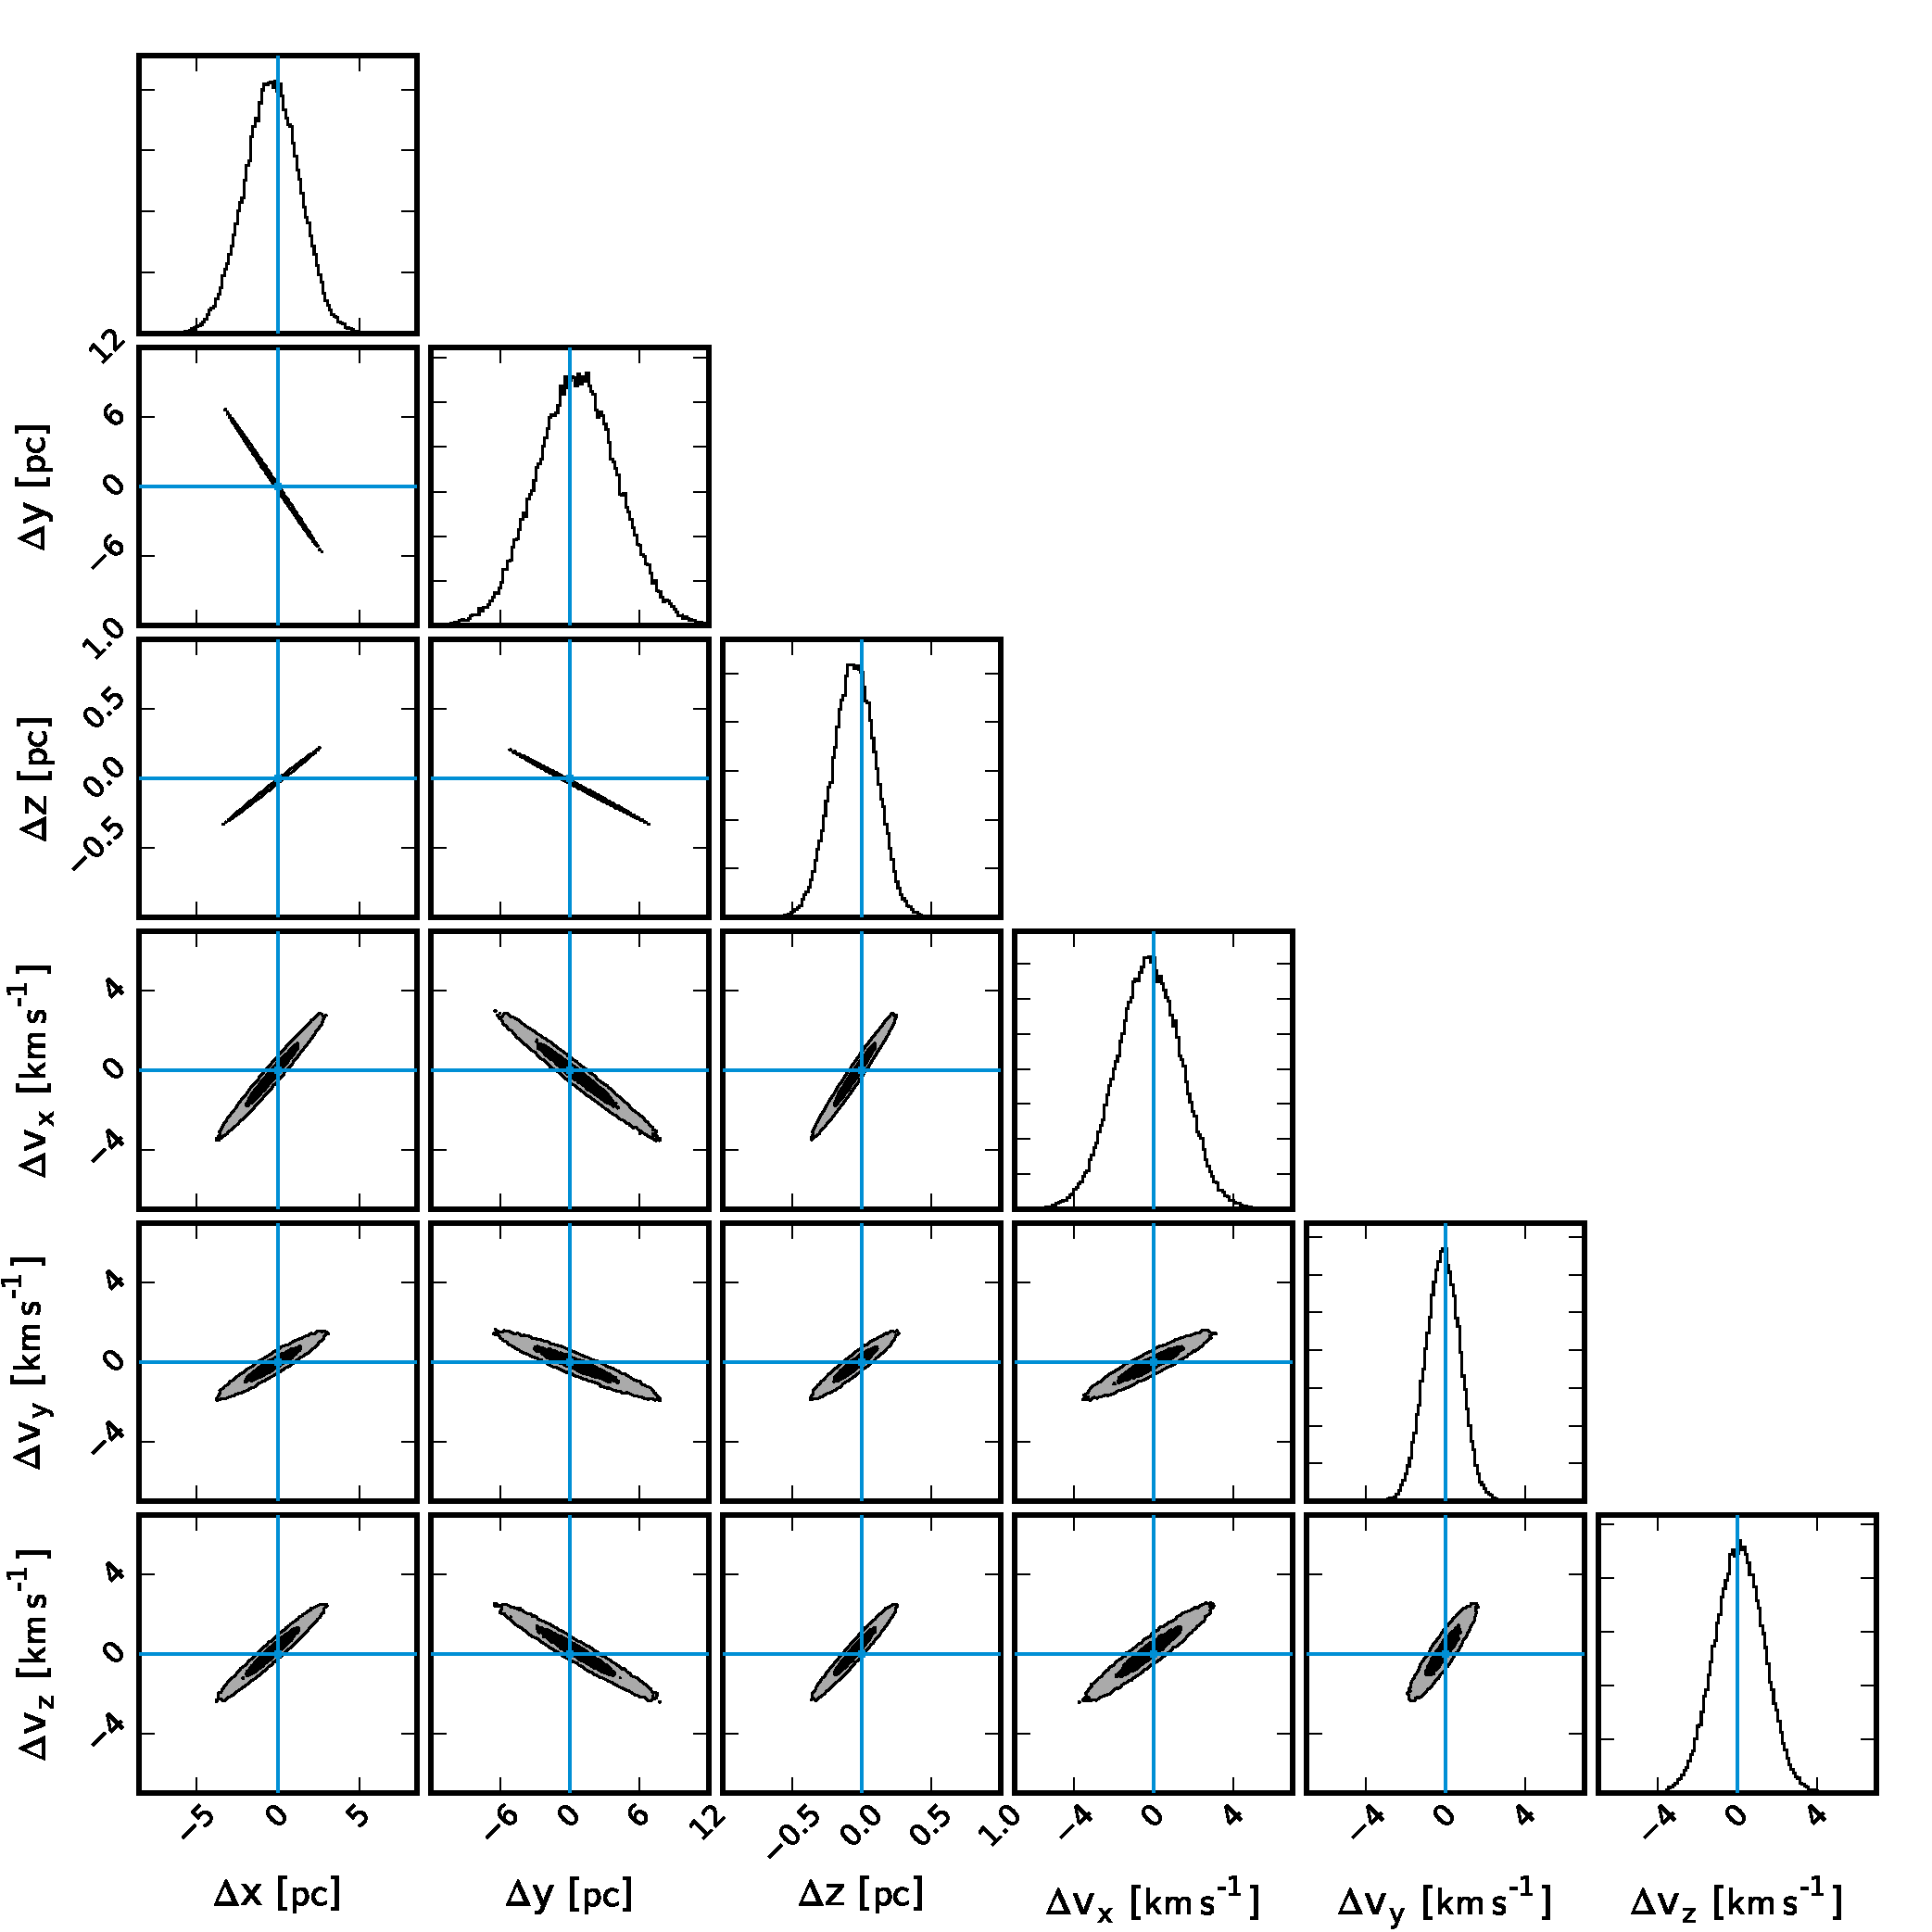
\includegraphics[width=\linewidth]{dx_dv_posterior.pdf}
  \end{center}
  \caption{%
    Differences in posterior samples over Galactocentric phase-space coordinates
    for the two stars \sunanalog\ and \bizarreone.
    \label{fig:dxdv}}
\end{figure}

\begin{figure}[htpb]
  \centering
  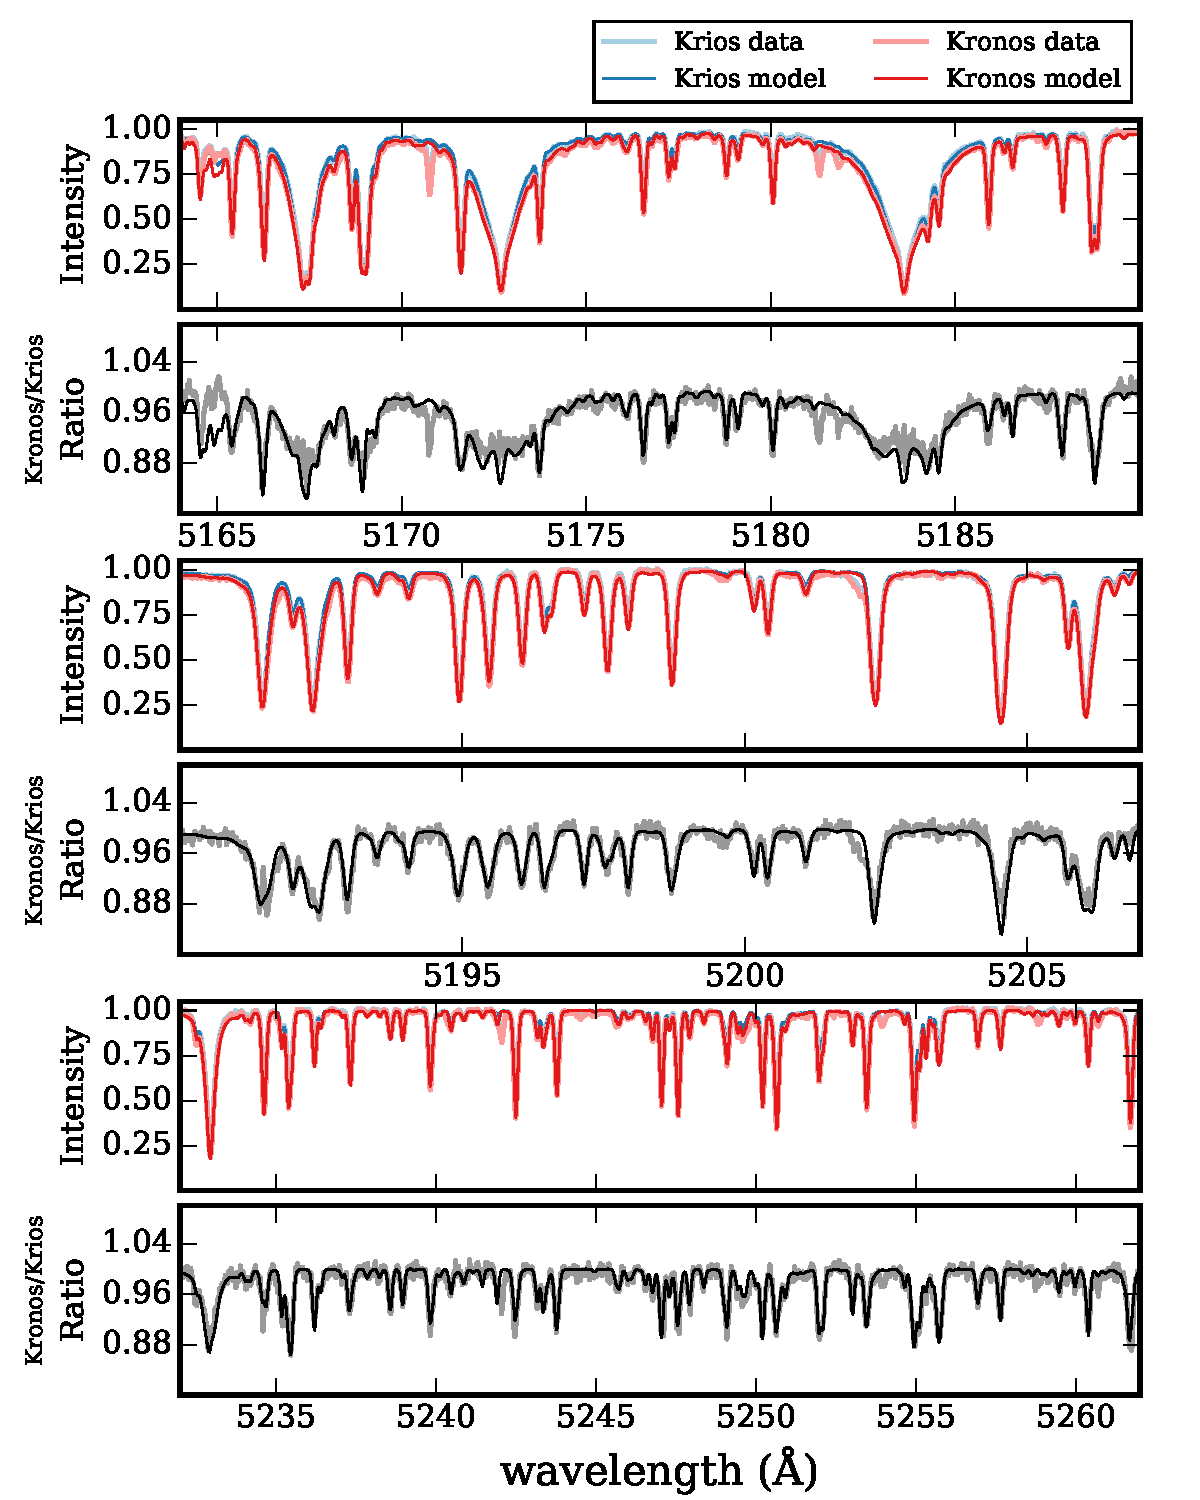
\includegraphics[width=0.95\linewidth]{spec1.pdf}
  \caption{Selective segments of the spectra of \sunanalog\ and \bizarreone.
    Alternating sets of two rows show
    the continuum-normalized data and model in the upper panel,
    and the ratio (\bizarreone/\sunanalog) of data (gray) and model (black)
    in the lower panel.
  }
  \label{fig:spec1}
\end{figure}

\begin{figure}[htpb]
  \centering
  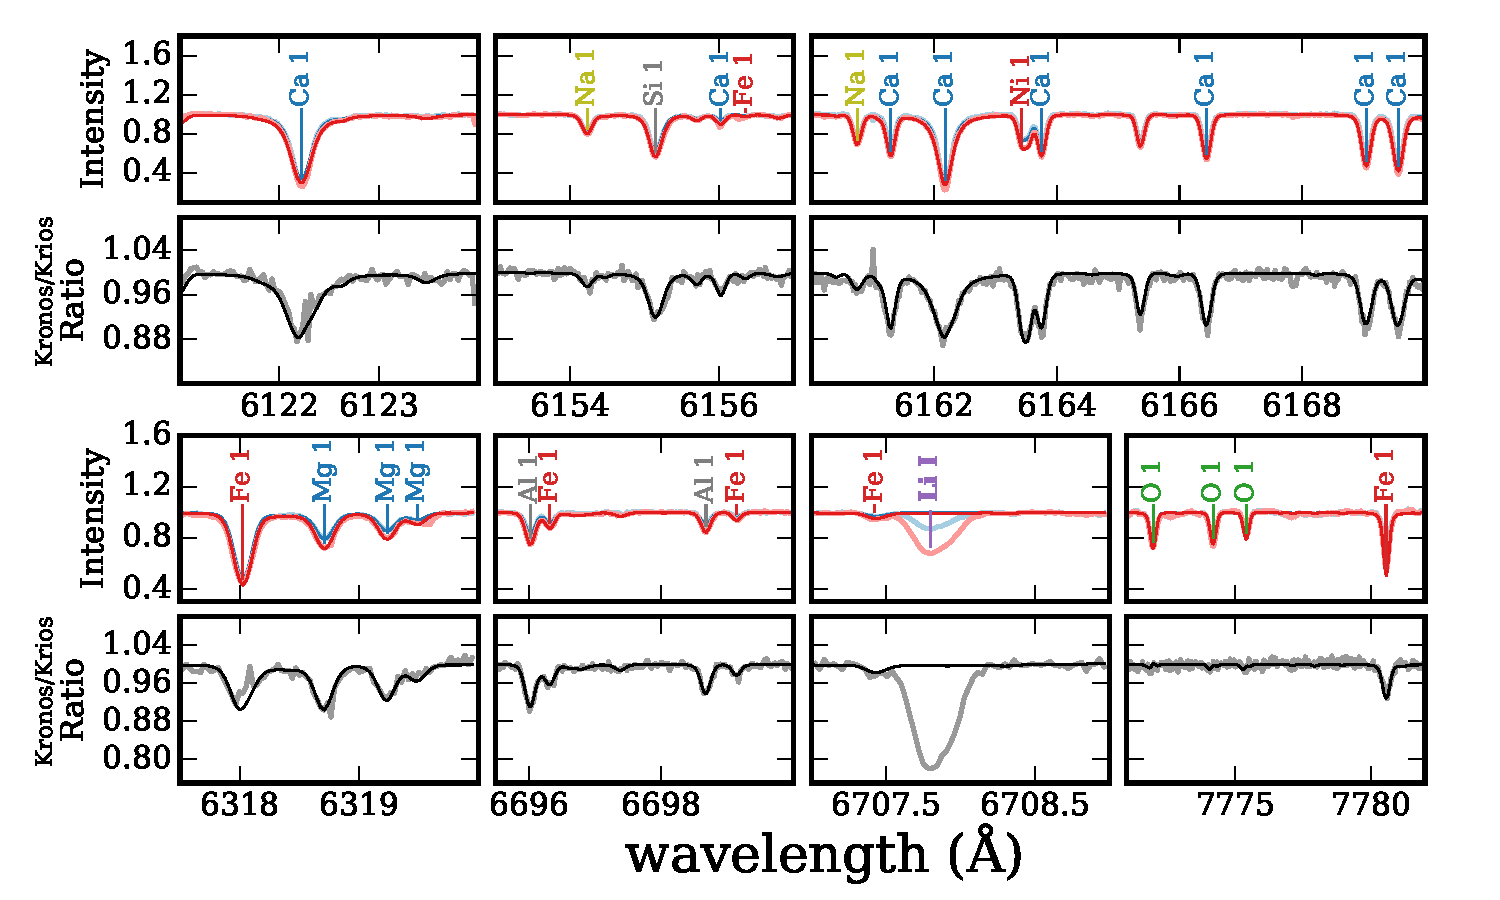
\includegraphics[width=0.95\linewidth]{spec2.pdf}
  \caption{Same as \figname~\ref{fig:spec1}
    but for smaller portions of spectra at longer wavelengths that are
    not dominated by \elem{Fe}.
    We mark elements that give rise to strong absorption lines.
    The feature in the third column of the second row is a strong \elem{Li}
    line that was not modeled by \citealt{2016ApJS..225...32B}; this line was
    studied in a separate work (\citealt{jmlithium}).
    Note that the lines of \elem{Na} and \elem{O}, which are under-enhanced
    in \bizarreone\ relative to \elem{Fe} or other refractory elements,
    show weaker residuals.
  }
  \label{fig:spec2}
\end{figure}

%TODO: plot styles...
\begin{figure}[htbp]
  \begin{center}
    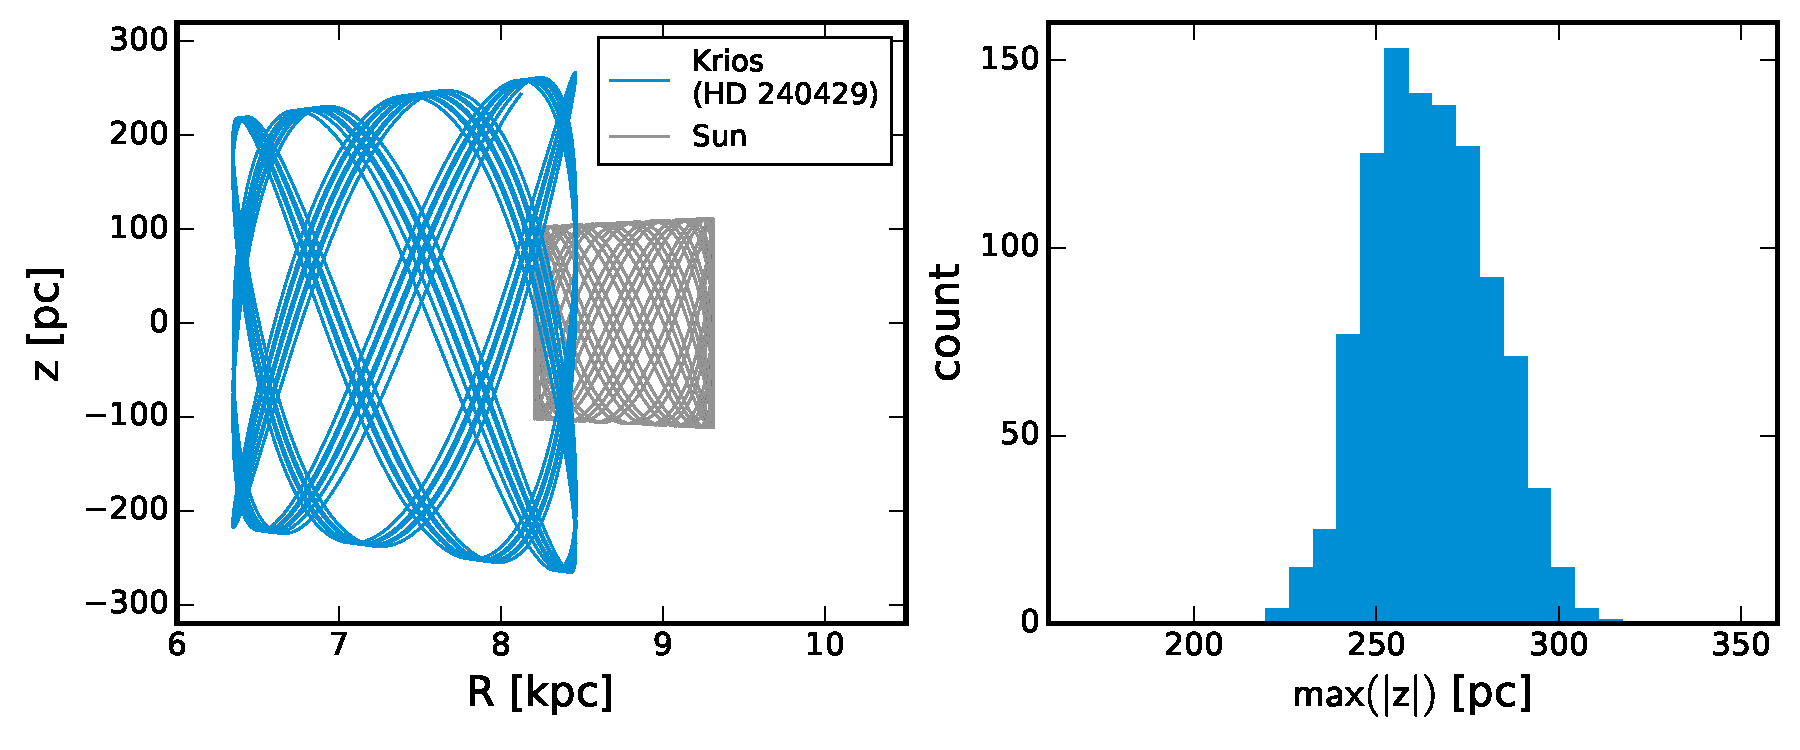
\includegraphics[width=\linewidth]{orbits.pdf}
  \end{center}
  \caption{Left panel: Galactic orbits computed for \sunanalog\ (black) and the
    Sun (grey).
    For \sunanalog, the initial conditions are set to the median of the
    posterior samples over the phase-space coordinates.
    The orbits are computed by integrating backwards from the present-day
    positions for $2.5$~Gyr with a time step of $0.5$~Myr using the Leapfrog
    integration scheme implemented in \project{Gala} (\citealt{gala}).
    Right panel: distribution of maximum $z$-heights for orbits computed from
    all posterior samples.
  }
  \label{fig:orbit}
\end{figure}
